\documentclass[a4paper,11pt]{article}
\usepackage{amsmath,amsthm,amsfonts,amssymb,amscd,amstext,vmargin,graphics,graphicx,tabularx,multicol} 
\usepackage[francais]{babel}
\usepackage[utf8]{inputenc}  
\usepackage[T1]{fontenc} 
\usepackage{pstricks-add,tikz,tkz-tab,variations}
\usepackage[autolanguage,np]{numprint} 

\setmarginsrb{1.5cm}{0.5cm}{1cm}{0.5cm}{0cm}{0cm}{0cm}{0cm} %Gauche, haut, droite, haut
\newcounter{numexo}
\newcommand{\exo}[1]{\stepcounter{numexo}\noindent{\bf Exercice~\thenumexo} : \marginpar{\hfill /#1}}
\reversemarginpar


\newcounter{enumtabi}
\newcounter{enumtaba}
\newcommand{\q}{\stepcounter{enumtabi} \theenumtabi.  }
\newcommand{\qa}{\stepcounter{enumtaba} (\alph{enumtaba}) }
\newcommand{\initq}{\setcounter{enumtabi}{0}}
\newcommand{\initqa}{\setcounter{enumtaba}{0}}

\newcommand{\be}{\begin{enumerate}}
\newcommand{\ee}{\end{enumerate}}
\newcommand{\bi}{\begin{itemize}}
\newcommand{\ei}{\end{itemize}}
\newcommand{\bp}{\begin{pspicture*}}
\newcommand{\ep}{\end{pspicture*}}
\newcommand{\bt}{\begin{tabular}}
\newcommand{\et}{\end{tabular}}
\renewcommand{\tabularxcolumn}[1]{>{\centering}m{#1}} %(colonne m{} centrée, au lieu de p par défault) 
\newcommand{\tnl}{\tabularnewline}

\newcommand{\bmul}[1]{\begin{multicols}{#1}}
\newcommand{\emul}{\end{multicols}}

\newcommand{\trait}{\noindent \rule{\linewidth}{0.2mm}}
\newcommand{\hs}[1]{\hspace{#1}}
\newcommand{\vs}[1]{\vspace{#1}}

\newcommand{\N}{\mathbb{N}}
\newcommand{\Z}{\mathbb{Z}}
\newcommand{\R}{\mathbb{R}}
\newcommand{\C}{\mathbb{C}}
\newcommand{\Dcal}{\mathcal{D}}
\newcommand{\Ccal}{\mathcal{C}}
\newcommand{\mc}{\mathcal}

\newcommand{\vect}[1]{\overrightarrow{#1}}
\newcommand{\ds}{\displaystyle}
\newcommand{\eq}{\quad \Leftrightarrow \quad}
\newcommand{\vecti}{\vec{\imath}}
\newcommand{\vectj}{\vec{\jmath}}
\newcommand{\Oij}{(O;\vec{\imath}, \vec{\jmath})}
\newcommand{\OIJ}{(O;I,J)}


\newcommand{\reponse}[1][1]{%
\multido{}{#1}{\makebox[\linewidth]{\rule[0pt]{0pt}{20pt}\dotfill}
}}

\newcommand{\titre}[5] 
% #1: titre #2: haut gauche #3: bas gauche #4: haut droite #5: bas droite
{
\noindent #2 \hfill #4 \\
#3 \hfill #5

\vspace{-1.6cm}

\begin{center}\rule{6cm}{0.5mm}\end{center}
\vspace{0.2cm}
\begin{center}{\large{\textbf{#1}}}\end{center}
\begin{center}\rule{6cm}{0.5mm}\end{center}
}



\begin{document}
\pagestyle{empty}
\titre{Interrogation sur les statistiques}{Nom :}{Prénom :}{Classe}{Date}

\begin{flushleft}
\begin{tabular}{|m{9.5cm}|m{1.25cm}|m{1.25cm}|m{1.25cm}|m{1.25cm}|m{1.25cm}|}
\hline 
\textbf{Compétences} & \begin{center}
\textbf{N.E.}
\end{center} & \begin{center}
\textbf{M.I.}
\end{center} & \begin{center}
\textbf{M.F.}
\end{center}  & \begin{center}
\textbf{M.S.}
\end{center} & \begin{center}
\textbf{T.B.M.}
\end{center} \\ 
\hline 
Je dois savoir  lire et interpréter des données sous forme de données brutes, de tableau, de diagramme (diagramme en bâtons, diagramme circulaire, histogramme) &  &  & & &\\
\hline 
Je dois savoir calculer des effectifs, des fréquences (liste, tableau, graphique, tableur) &  &  & & &\\
\hline
Je dois savoir calculer une moyenne pondérée &  &  & & &\\
\hline
\end{tabular} 
\end{flushleft}

\textit{N.E = Non évalué ; M.I. = Maîtrise insuffisante ; M.F. = Maîtrise fragile ; M.S. = Maîtrise satisfaisante ; T.B.M. = Très bonne maîtrise}\\

\exo{10}

L'histogramme ci-dessous donne la répartition des élèves d'un collège en fonction du temps qu'ils mettent à venir au collège. 

\begin{center}
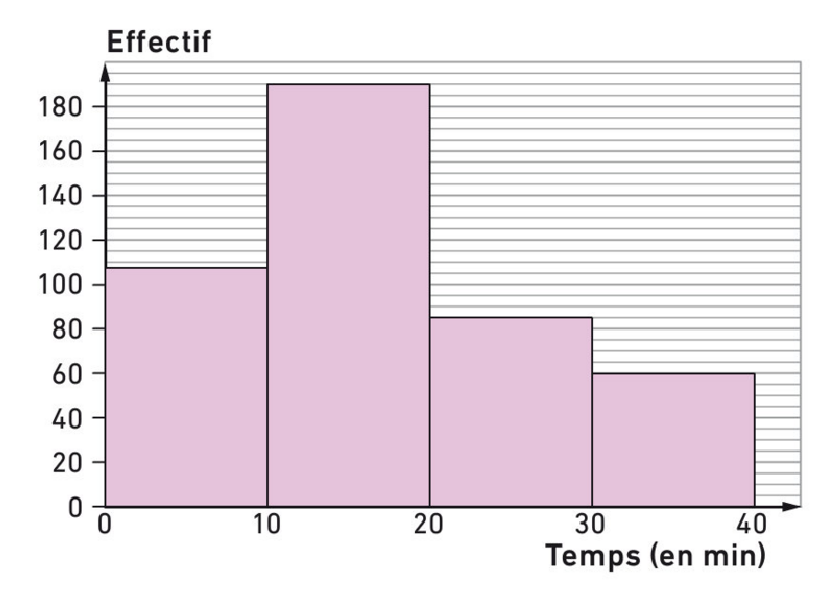
\includegraphics[scale=0.8]{interro2.eps} 
\end{center}

Voici un tableau qui représente la situation :\\

\renewcommand{\arraystretch}{2}

\begin{tabular}{|c|c|c|c|c|}
\hline 
Temps (en min) & \hspace*{0.5cm} [0;10[  \hspace*{0.5cm} &  \hspace*{0.5cm} [10;20[  \hspace*{0.5cm} &  \hspace*{0.5cm} [20;30[  \hspace*{0.5cm}& \hspace*{0.5cm} [30;40[  \hspace*{0.5cm}\\ 
\hline 
Effectifs &  &  &  &   \\ 
\hline 
Effectifs cumulés croissants &  &  &  &   \\ 
\hline 
Fréquences (en pourcentage) &  &  &  &    \\ 
\hline 
\end{tabular} 

\vspace*{0.4cm}


\q Compléter la ligne des effectifs et des effectifs cumulés du tableau ci-dessus. (sans justification)\\

\q Combien d'élèves mettent plus de 10 minutes, \textit{(10 min inclus), } pour venir au collège ? \\

\q Quel est l'effectif total de ce collège ? \\


\q Quelle est la fréquence en pourcentage du nombre d'élèves qui ont un temps de trajet entre 0 et 10 min à venir au collège ?  \\

\q Compléter la ligne des fréquences en pourcentage. (sans justification)\\


\q Quelle est la fréquence en pourcentage du nombre d'élèves qui mettent au plus 30 minutes, \textit{(30 minutes exclu)}, pour aller au collège ? \\


\q Quelle est la moyenne du temps de trajet des élèves de ce collège ? \\

\noindent  \reponse[36]\\ 
   

\end{document}
